% !TEX root = main.tex

\section{Introduction}
A \emph{knowledge graph} (KG) is a heterogeneous graph structure that captures knowledge encoded in a form of {\em head--relation--tail} triples, where the {\em head} and {\em tail} are two entities (\ie, nodes) and the {\em relation} is an edge between them (\eg, {\em (Paris, CapitalOf, France)}).
Knowledge graphs form the backbone of many AI systems across a wide range of domains: recommender systems~\citep{wang2018dkn,ying2018graph,wang2019knowledge,wu2019dual}, question answering~\citep{berant2013semantic,sun2018open,sun2019pullnet,saxena2020improving,ren2021lego},  commonsense reasoning~\citep{lin2019kagnet,feng2020scalable,yasunaga2021qa,lv2020graph}, personalized medicine~\cite{ruiz2021identification} and drug discovery~\cite{zitnik2018modeling,drkg2020}.

Reasoning over such KGs consists of two types of tasks: (1) single-hop link prediction (also known as knowledge graph completion), where given a {\em head} and a {\em relation} the goal is to predict one or more {\em tail} entities. For example, given {\em TuringAward--Win--?} (\ie, Who are the Turing Award winners?), the goal is to predict entities {\em GeoffHinton, DonKnuth}, etc.; %
And, (2) multi-hop reasoning, where one needs to predict (one or many) of the {\em tails} of a multi-hop logical query. For example, answering ``Who are co-authors of Canadian Turing Award winners?'' (\Figref{fig:background}(A))).
Finding answers to such query requires imputation and prediction of multiple edges across two parallel paths, while also using logical set operations (\eg, intersection, union). \Figref{fig:background}(B) shows the query computation plan and to determine the entities that are the answers to such a complex multi-hop query, missing links typically need to be implicitly inferred \Figref{fig:background}(C).
%
Notice that both tasks are closely related to each other. Knowledge graph completion can be viewed as a special case of a multi-hop reasoning task when the query consists of a single relation (\eg, {\em France--CapitalOf--?}). Multi-hop reasoning is a strict generalization of knowledge graph completion with much broader applicability but with its own set of unique computational and scalability challenges. 

Currently there are no frameworks that support multi-hop reasoning on massive Knowledge graphs. For example, among many recent works on multi-hop reasoning~\citep{hamilton2018embedding,ren2020query2box,ren2020beta,sun2020faithful,guu2015traversing,das2017chains,chen2021fuzzy,liu2021neural,kotnis2020answering,zhang2021cone,choudhary2021probabilistic} the largest KG used has only 63K entities and 592K relations.
%
Moreover, while there are scalable frameworks for single-hop KG completion~\citep{zhu2019graphvite,lerer2019pytorch,zheng2020dgl,pgl,mohoney2021marius}, such frameworks cannot be directly used for multi-hop reasoning due to the more complex nature of the multi-hop reasoning task.


Scaling up embedding-based multi-hop KG reasoning methods is a critical need for many real-world AI applications and remains largely unexplored. Two significant challenges exist: (1) on the algorithmic side, given a massive KG (with hundreds of millions of entities), it is no longer feasible to materialize training instances, and training data needs to be efficiently sampled on the fly with a high throughput to ensure GPUs are fully utilized. And (2), on the system side, recent single-hop large-scale KG embedding frameworks are based on graph-partitioning~\citep{zhu2019graphvite,lerer2019pytorch,zheng2020dgl,mohoney2021marius} which is problematic for multi-hop reasoning. Multi-hop reasoning requires traversing multiple relations in the graph, which will often span across multiple partitions.

\begin{figure}[t]
\centering
    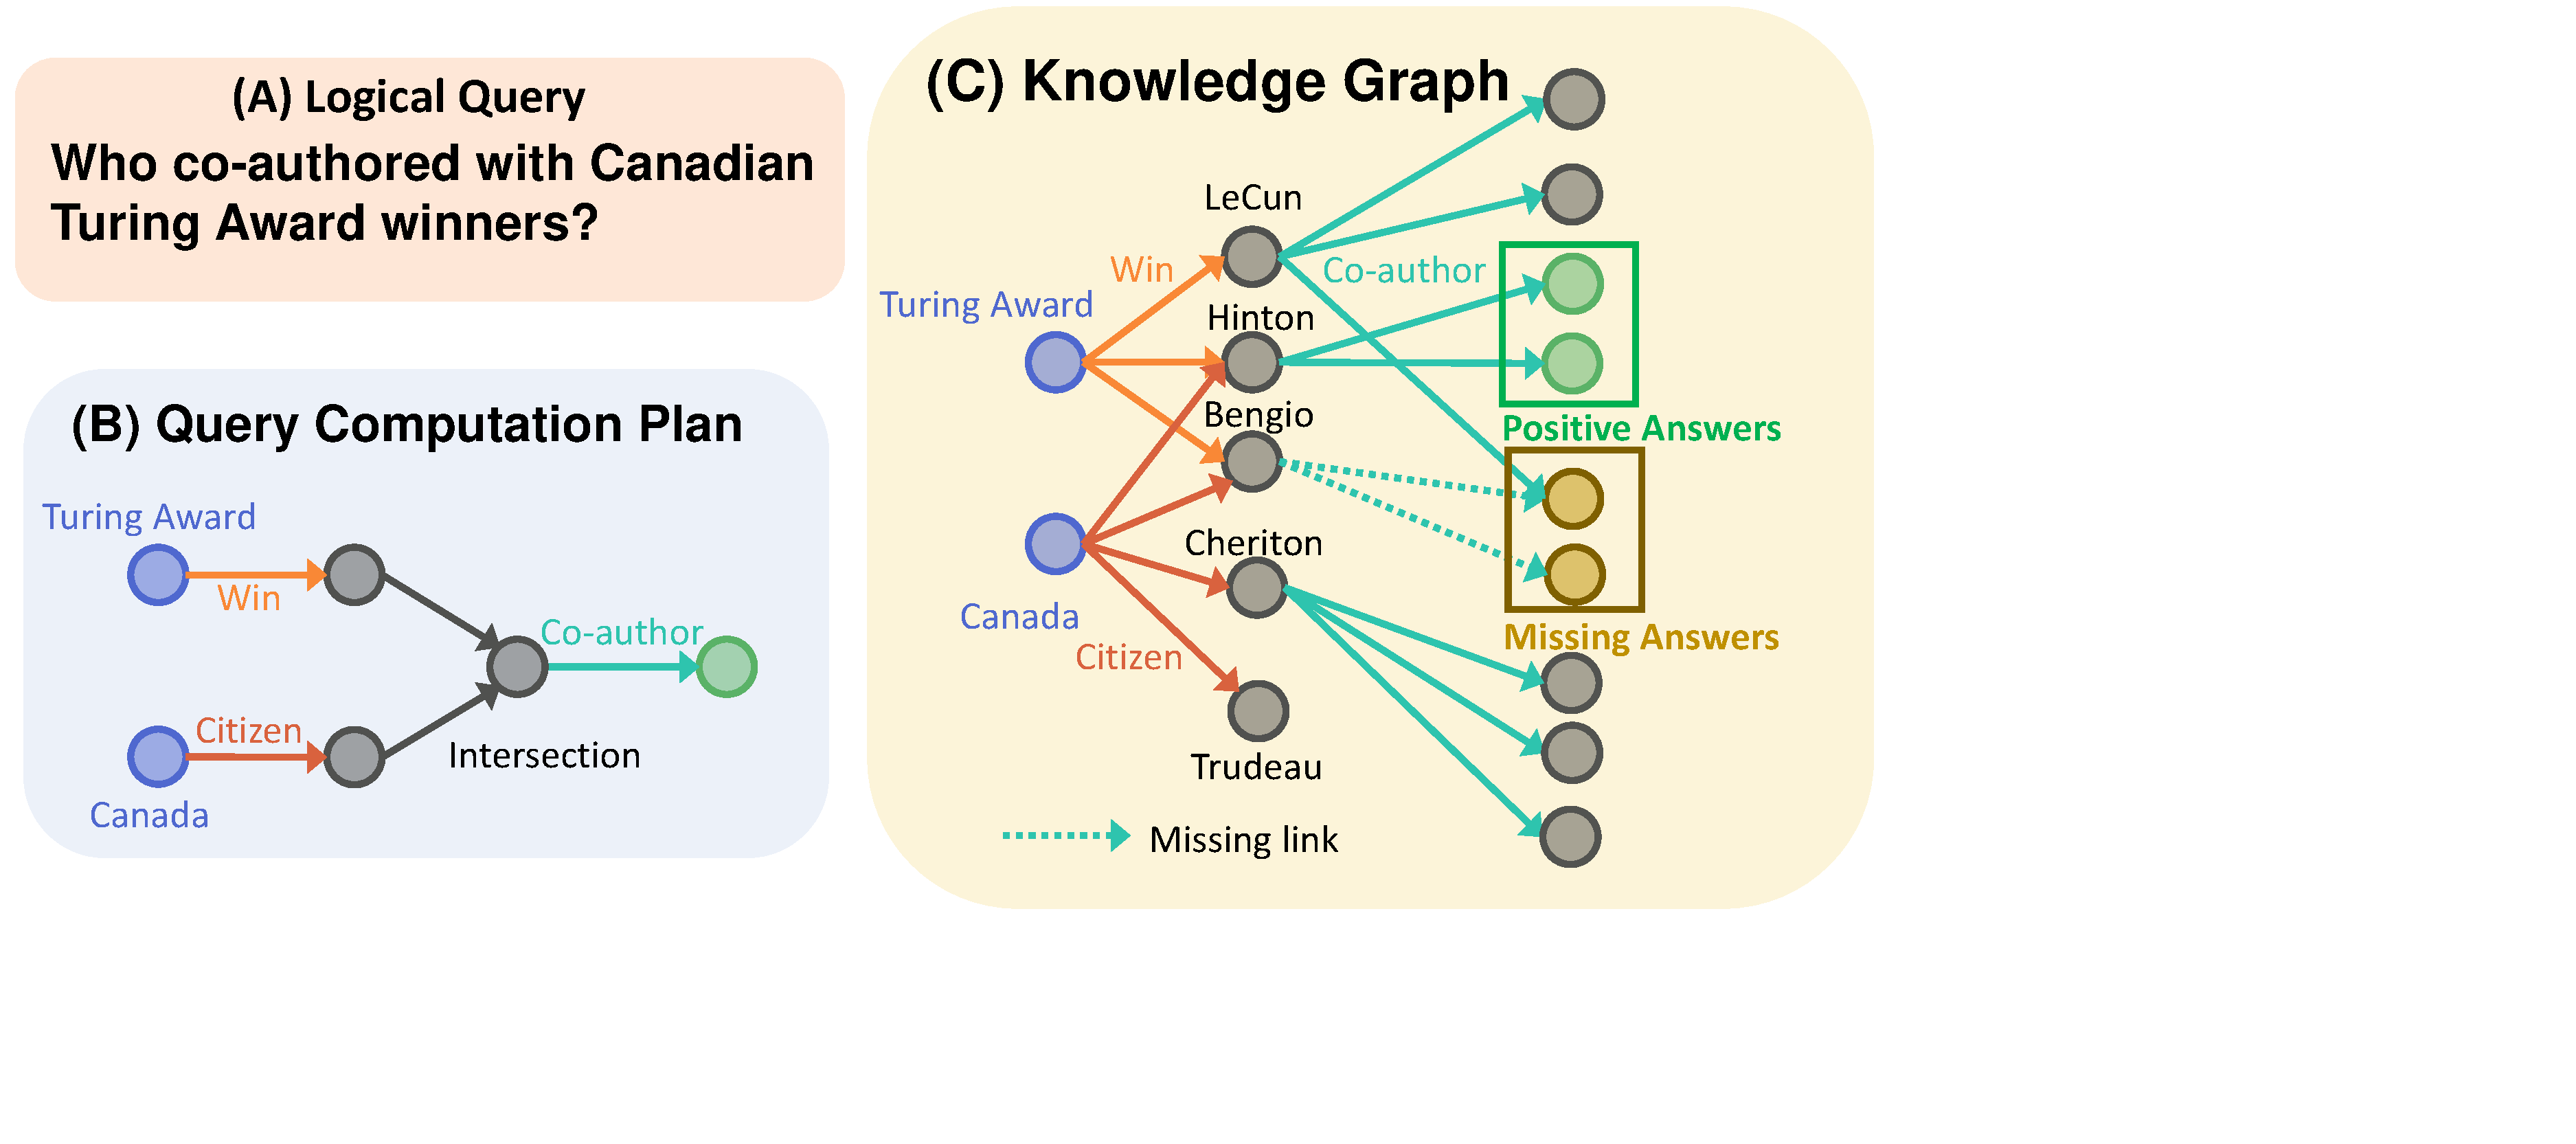
\includegraphics[width=0.45\textwidth]{figs/background.pdf}
    \caption{Query embedding methods aim to answer multi-hop logical queries (A) by avoiding explicit knowledge graph traversal and executing the query directly in the embedding space by following the query computation plan (B). Such methods are robust against missing links (C).
    }
    \vspace{-1mm}
\label{fig:background}
\end{figure}

To combat these challenges, we propose \emph{\modellong~(\modelshort)}, the \emph{first general framework} for single- and multi-hop reasoning on massive KGs. %
\modelshort performs algorithm-system co-optimization for scalability. \textbf{On the algorithmic side}, the key is to efficiently generate training examples online. To generate a training example with a set of positive and negative entities, we first instantiate a query on a given KG (\Figref{fig:query}(B)) from a set of query logical structures (\Figref{fig:query}(A)). The root of the instantiated query represents a known positive (answer) entity.
To obtain a set of negative entities (non-answers), 
n\"aive execution of the query computation plan (\Figref{fig:background}(B))
using KG traversal (\Figref{fig:background}(C)) to identify positive/negative entities has exponential complexity with respect to the number of hops of the query.
Therefore, we propose a bidirectional rejection sampling approach to efficiently obtain high-quality negative entities for the instantiated queries.  
The key insight of the training data sampler is to identify the \emph{optimal node cut} (red node in~\Figref{fig:query}(C)) of the computation plan via dynamic programming, then performing forward KG traversal (\Figref{fig:query}(C)) as well as backward verification (\Figref{fig:query}(D)) simultaneously, hence bidirectional rejection sampling. 
The nodes in the optimal cut cache the intermediate results from the forward KG traversal; for backward verification, we propose positive and negative candidate entities, traverse backward to the optimal cut and perform rejection sampling based on the overlap of the forward and backward sets. This reduces the worst case complexity by a square root, which makes it feasible to generate a training query, a positive answer entity and negative non-answer entities on the fly. 

\textbf{On the system side}, \modelshort operates on the full KG directly in a shared memory environment with multiple GPUs, while storing embedding parameters in the CPU memory to overcome the limited GPU memory. This design choice bypasses the potential drawbacks of graph partitioning for multi-hop reasoning in current KG embedding systems, but also brings efficiency challenges. We design an asynchronous scheduler to maximize the throughput of GPU computation, via overlapping sampling, asynchronous embedding read/write, neural network feed-forward, and optimizer updates, as depicted in Figure~\ref{fig:pipeline}. 
As a result, we obtain an efficient implementation that can achieve near linear speed-up with respect to the number of GPUs.

We demonstrate the scalability of \modelshort on three multi-hop reasoning algorithms (GQE~\citep{hamilton2018embedding}, Q2B~\citep{ren2020query2box}, BetaE~\citep{ren2020beta}), six single-hop KG completion approaches (TransE~\citep{bordes2013translating}, RotatE~\cite{sun2019rotate}, DistMult~\cite{yang2014embedding}, ComplEx~\cite{trouillon2016complex}, Q2B~\citep{ren2020query2box} and BetaE~\citep{ren2020beta}) on six different benchmark KGs. The largest is the Freebase KG~\cite{bollacker2008freebase,zheng2020dgl} that contains 86M nodes and 338M edges, which is about 1,500 times larger than the largest KG previously considered for multi-hop reasoning. The new sampling technique improves the worst case runtime of enumerative search by 4 orders of magnitude. On small KGs, \modelshort{} runs 2.2 times faster with 30.6\% less GPU memory usage compared to the existing (non-scalable) multi-hop reasoning framework~\citep{kgreasoning}. 
\modelshort also supports single-hop reasoning. Here \modelshort achieves comparable or even better efficiency with state-of-the-art frameworks (which do not support multi-hop reasoning) on both single-GPU and multi-GPU settings.

\modelshort can be easily deployed in a single-machine environment with a minimum requirement on the capacity of GPU memory. For example, it uses less than 2GB GPU memory when training a 400 dimensional embedding on the Freebase KG with 86M entities. \modelshort's throughput scales nearly linearly with the number of GPUs. 
%  
\modelshort also provides an easy-to-use interface where implementing a new embedding model takes less than 50 lines of code. Together with the benchmarks, \modelshort provides a test bed for accelerating future research in multi-hop reasoning on KGs. \modelshort is open sourced at \url{https://github.com/google-research/smore}.
